\begin{frame}{What is an Adversarial Example?}
  \onslide<+->{}
  \onslide<+->{
    \begin{definition}
      \textbf{\blue{Adversarial Example}}: Input chosen/modified by an adversary that is almost \textit{indistinguishable} from natural data but is (\textit{confidently}) misclassified by the model.
    \end{definition}
  }

  \begin{columns}
    \begin{column}{0.23\textwidth}
      \onslide<+->{
        \begin{center}
          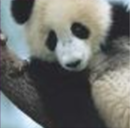
\includegraphics{adv_panda}

          \textbf{\green{Prediction}}
          \\
          \textbf{Panda}
          \\
          55.7\% Confidence~\cite{Goodfellow:2014}
        \end{center}
      }
    \end{column}
    \onslide<+->{
      \begin{column}{0.05\textwidth}
          \begin{center}
            +\vspace{1.6cm}
          \end{center}
      \end{column}
      \begin{column}{0.20\textwidth}
          \begin{center}
            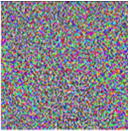
\includegraphics{adv_noise}

            \textbf{\green{Prediction}}
            \\
            \textbf{Nematode}
            \\
            8.2\% Confidence
          \end{center}
      \end{column}
    }
    \onslide<+->{
      \begin{column}{0.05\textwidth}
          \begin{center}
            =\vspace{1.6cm}
          \end{center}
      \end{column}
      \begin{column}{0.20\textwidth}
          \begin{center}
            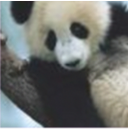
\includegraphics{adv_combined}
            \textbf{\green{Prediction}}
            \\
            \textbf{Gibbon}
            \\
            99.3\% Confidence
          \end{center}
      \end{column}
    }
    \onslide<+->{
      \begin{column}{0.20\textwidth}
          \begin{center}
            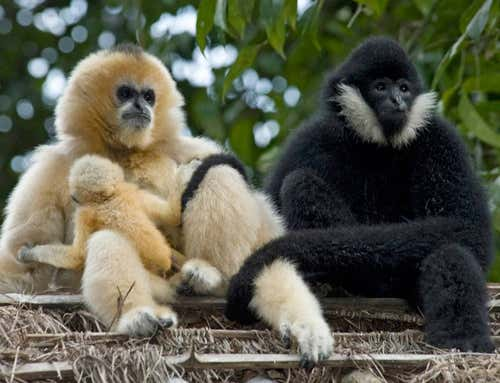
\includegraphics[scale=0.15]{gibbon}
            \textbf{\red{Actual}\\Gibbon}
          \end{center}
      \end{column}
    }
  \end{columns}

\end{frame}


\begin{frame}{Attack Paradigms}
  \madry\ study adversarial robustness under two different attack paradigms:
  \vfill
  \begin{enumerate}[<+->]
    \item \blue{\textbf{Black-Box}}: Adversary has no direct access to target network
      \begin{itemize}[<+->]
        \setlength\itemsep{6pt}
        \item \red{Weaker} attack paradigm
        \item Adversary may have \textit{rough} information, e.g.,~model architecture \& training dataset
          \begin{itemize}[<+->]
            \setlength{\itemsep}{6pt}
            \item \textit{Example}: Transfer attack
            \item \textbf{Question}: What is a transfer attack? What is an intuition for why they are effective?
          \end{itemize}
        % \item Generally \textit{one-shot} attacks
      \end{itemize}

    \vfill
    \item \blue{\textbf{White-Box}}: Adversary has access to target network's parameters
      \begin{itemize}
        \setlength\itemsep{6pt}
        \item \green{Stronger} attack paradigm
        \item \textit{Examples}: PGD and FGSM (both discussed in this talk)
        \item Enables \textit{iterative} attacks, e.g.,~refined probing
      \end{itemize}
  \end{enumerate}
\end{frame}
